\section{Software correlator}\label{sec:vlbi}
If the data in an {\it e}-VLBI experiment can be streamed over the
internet to JIVE, it can also be sent to another correlator. Within
\scarie, we are investigating the possibilities of a next generation
correlator using a computing Grid. The advantages of a software
correlator over a new dedicated hardware correlator lie in its
flexibility and accuracy. The software correlator can be tuned for
special experiments. The main advantage of a dedicated hardware
correlator is the greater performance. The advance of general purpose
computing is making software correlation a cost-effective solution for
a range of applications. A similar approach is presented in
\cite{deller-2007}.

The flexibility of its architecture allows the software correlator to
change with the needs of researchers. In fact, the first version of
the software correlator was developed to track the Huygens spacecraft
during its descent through the atmosphere of Saturn's moon Titan. Due
to the nature of this experiment, special requirements are put on the
correlator, which the current hardware correlator is not able to
provide.  Moreover, we expect that the costs of developing a software
correlator are much lower than the costs for a hardware correlator.

Computationally the correlation is relatively inexpensive, in the
sense that it requires only few operations per transferred bytes.
However, due to the high data rates, the absolute number of clock
cycles required by the application is still extremely high. Moreover,
the problem is quadratic in the number of telescopes participating in
the experiment since it is linear in the number of channel pairs that
have to be correlated. The huge need for networking and computing
power makes a computing Grid an ideal platform for this application.

In the software correlator, we split the computation in time slices.
These time slices are processed in parallel (see
Figure~\ref{fig:netw_corr}). The signal from a telescope is received
by a single so-called input node.  The input node sends slices of data
to one of the available correlator nodes. The correlator node receives
data from all telescopes for a certain time slice and performs the
correlation. The size of the output of the correlation is much smaller
than the input size and can be collected and stored by a single output
node.  There is a single manager node that assigns data to available
computing nodes.



\begin{figure}
  \centering
  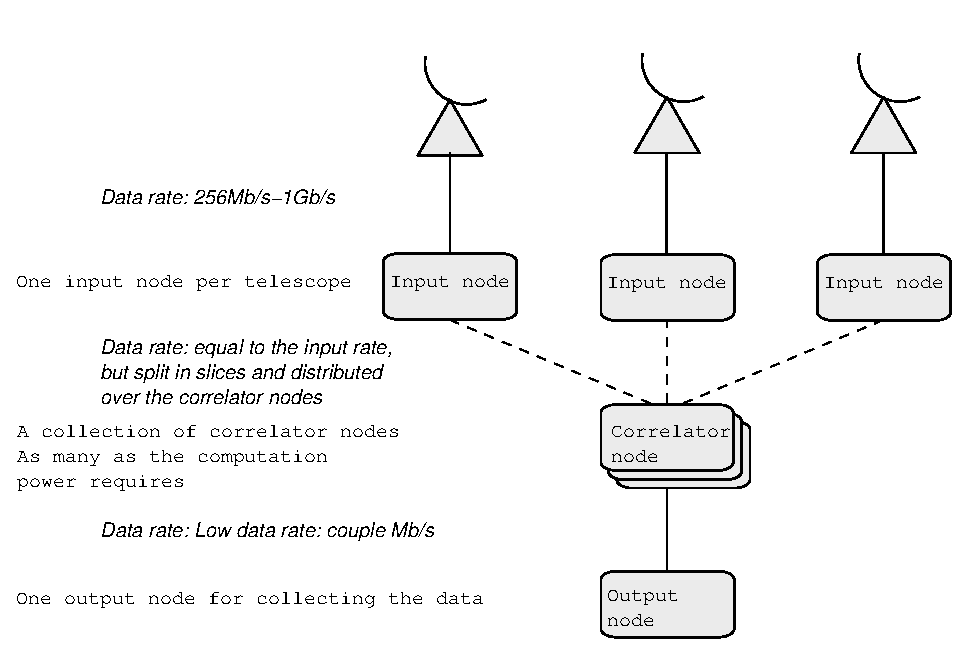
\includegraphics[width=.75\textwidth]
    {img/Network_correlator}
    \caption{Outline of the network connections between different
      components in the software correlator.}
  \label{fig:netw_corr}
\end{figure}


\subsection{Design}
The software correlator is written in \verb~C++~ and uses several
standard libraries like \verb~fftw~ \cite{FFTW05} for the fast Fourier
transforms, \verb~mpich~ \cite{Gropp:1996:HPI} as the MPI
implementation , \verb~GSL~ \cite{GSL} for cubic spline fitting and
the standard template library.

At start up, the manager node is created, which starts the other nodes
and connects them. The manager node is the central node that controls
the workflow of the entire software correlator. It assigns time slices
to available correlator nodes and handles errors. After all time
slices are processed it terminates the software correlator.

The input node receives the data from a data stream, which can either
be a file, a TCP connection or directly from the dedicated hardware
used to record and play back the data. On request of the manager node,
it can extract the current time from the data stream or go to a
specified time. When the input node gets a request to send data for a
certain time slice to a correlator node, it seeks the right starting
sample in the input stream and sends the data to the correlator node.

The correlator node gets data for the same time slice from every input
node. Before the signal can be correlated, the integer delay corrected
signal has to be processed further. First, the signal is delayed by a
the fractional delay that remains after the integer delay done in the
input node. After that a phase correction is done, which is a first
order approximation of the delay function. These manipulations are not
done on the input node because they require floating point samples,
hence the data stream expands from 2 bits per sample to 32 bits or
even 64 bits per sample, which would require much more network
bandwidth. After the fractional delay and the phase rotation, the
signal is ready to be correlated. The auto and cross correlation are
then computed by Fourier transforming the input signal and
element-wise multiplying all combination of telescope-pairs. These
values are accumulated over a certain period of time and the
accumulated values are sent to the output node.

The output node will receives the data from the correlator nodes,
sorts the data and stores it at a specified location.

\subsection{Network connections}
Since correlation is mainly a networking problem, testing and
optimizing the data flows is of vital importance for the performance
of the software correlator. We distinguish two types of data flows:
containing control messages and the signals from the telescopes. 

\paragraph{Control messages}
The control messages are sent between different nodes to regulate the
correlation. They form a low bandwidth stream and MPI is used to send
these messages. The network is mainly star shaped around the control
node, but there are some connections during the initialization between
input nodes and the correlator nodes and between correlator nodes and
the output node. Since the messages control the correlator, the
delivery of the messages has to be guaranteed. For the analysis of the
network throughput these messages are of no importance.

\paragraph{Signal of the telescopes}
The signal from the telescopes requires far more bandwidth than the
control messages. The constant throughput for these connections is
very important as we are dealing with real time data. Some packet loss
is even acceptable if a data stream at a constant rate can then be
maintained. The connections for these data streams are set up to be
exchangeable such that it is possible to test different network
protocols like TCP (using jumbo frames), or protocols used for
streaming media. The network consists of three layers: from the
telescopes to the data nodes, then to the correlator nodes and finally
to the output node, as is shown in
Figure~\ref{fig:netw_corr}.\marginpar{NGHK: mention StarPlane}



%%% Local Variables:
%%% mode: latex
%%% TeX-master: "Ingrid"
%%% End:
